In this section we consider zero-value seller settings when the buyer's valuation distribution is assumed to be MHR. With this stronger assumption that the distribution is MHR rather than regular, we are able to improved the GFT approximation and show that the approximation for \emph{all} instances with MHR distributions is strictly larger than the approximation guaranteed by regularity alone.


\begin{restatable}{theorem}{thmGFTmhrbuyer}
\label{thm:improved GFT:mhr buyer} 
    For every bilateral trade instance of a zero-value seller and buyer with MHR valuation distribution $\buyerdist$, there exists price $\fprice$ smaller than the monopoly reserve $\optreserve$ for distribution $\buyerdist$,\footnote{When distribution $\buyerdist$ is MHR, its induced monopoly reserve $\optreserve$ is unique.} 
    such that the {\FixPrice} mechanism with trading price $\fprice$ is {\ksfair} and its GFT is at least $\calC$ fraction of the {\SecondBest} $\OPTSB$. Here $\calC$ is the solution to minimization program~\ref{program:GFT:mhr buyer},  
    and we observe that 
    $\calC\geq \fixedPriceGFTPercentageMHR$ by a numerical computation.

    Moreover, there exists an instance of a zero-value seller and buyer with MHR valuation distribution, in which any BIC, IIR, ex ante WBB mechanism that is {\ksfair} has GFT that is less than  $\fixedPriceGFTPercentageUBMHR$ of the {\SecondBest} $\OPTSB$.
\end{restatable}

\Cref{thm:improved GFT:mhr buyer} directly follows \Cref{lem:GFT program:mhr buyer,lem:GFT UB:mhr buyer} which are presented below. Their proofs are similar to the ones for regular distributions in \Cref{subsec:improved GFT:regular buyer}. 


\subsubsection{GFT Approximation by KS-Fair {\FixPrice}}

In this section we show that {\FixPrice} that is {\ksfair} can get very good GFT approximation. We characterize the GFT approximation of a {\ksfair} {\FixPrice} in the following lemma. Its proof is similar to the one for \Cref{lem:GFT program:regular buyer} in \Cref{subsec:improved GFT:regular buyer}. Specifically, we search over all MHR distributions and argue that the worst GFT can only be induced by a subclass of them, whose \emph{cumulative hazard rate function} (rather than the revenue curve, as was the case for regular buyer distributions) can be characterized by finite many parameters (see \Cref{fig:GFT program:mhr buyer}). We defer its formal proof to \Cref{apx:lemgftprogrammhrbuyer}.

\begin{figure}
    \centering
    \begin{tikzpicture}[scale=1, transform shape]
\begin{axis}[
axis line style=gray,
axis lines=middle,
xtick={0, 0.4, 0.8, 1, 1.22436, 1.64872, 2.7182818},
ytick={0, 0.1177216, 0.5, 2.1},
xticklabels={0, $\val_0$, $\price$, 1, $\val_1$, $\optreserve$, $e$},
yticklabels={0, $\ln(\frac{\price}{\revratio})$, $\ln(\optreserve)$, $\infty$},
xmin=0,xmax=3.0,ymin=-0.05,ymax=2.9,
width=0.8\textwidth,
height=0.5\textwidth,
samples=500]

% \fill[blue!20] (0,0) -- (0.642857, 0.229591877551) -- (0.725, 0.199375) -- cycle;





\addplot[domain=1:5, dashed, line width=0.5mm] (x, {ln(x)});


\addplot[dotted, gray, line width=0.3mm] (1.64872, 0) -- (1.64872, 0.5) -- (0, 0.5);

\addplot[dotted, gray, line width=0.3mm] (0.8, 0) -- (0.8, 2.4);

\addplot[dotted, gray, line width=0.3mm] (1.64872, 2.1) -- (1.64872, 2.4);
\addplot[dotted, gray, line width=0.3mm] (0.8, 0.1177216) -- (0., 0.1177216);

\addplot[dotted, gray, line width=0.3mm] (1.22436, 0) -- (1.22436, 0.242612);

\addplot[dotted, gray, line width=0.3mm] (1.64872, 2.1) -- (0, 2.1);


\addplot[red, line width=0.5mm] (0, 0) -- (0.4, 0) -- (1.22436, 0.242612);
\addplot[domain=1.22436:5, red, line width=0.5mm] (x, {0.5 - 1 / 1.64872 * (1.64872 - x)});


\addplot[blue, line width=0.5mm] (0, 0) -- (0.8, 0.1177216) -- (1.64872, 0.5);
\addplot[blue, dotted, line width=0.5mm] (1.64872, 0.5) --(1.64872, 2.1);
\addplot[blue, line width=0.5mm] (1.64872, 2.1) --(5, 2.1);
\draw[blue, fill=white, line width=0.5mm] (axis cs:1.64872, 2.1) circle[radius=0.05cm];


\addplot[domain=0:5, black!100!white, line width=0.5mm] (x, {x * x * 0.18394});



\draw[decorate,decoration={brace,amplitude=8pt}] (0.0,2.4) -- (0.8,2.4) node[midway,above=6pt] {$L$/{{\color{red}$\LOverBar$}}/{{\color{blue}$\LUnderBar$}}};
\draw[decorate,decoration={brace,amplitude=8pt}] (0.8,2.4) -- (1.64872,2.4) node[midway,above=6pt] {$M$/{{\color{red}$\MOverBar$}}/{{\color{blue}$\MUnderBar$}}};
\draw[decorate,decoration={brace,amplitude=8pt}] (1.64872,2.4) -- (3,2.4) node[midway,above=6pt] {$H$/{{\color{red}$\HOverBar$}}/{{\color{blue}$\HUnderBar$}}};

\end{axis}

\end{tikzpicture}
    \caption{Graphical illustration of the analysis for \Cref{lem:GFT program:mhr buyer}. The black curve is the convex cumulative hazard rate function $\cumhazard$ of the buyer. The red and blue cumulative hazard rate functions $\cumhazard_1, \cumhazard_2$ (defined in the analysis) sandwich the original cumulative hazard rate function $\cumhazard$. The black dashed line is $\ln(\val)$, which touches the cumulative hazard rate function $\cumhazard$ at monopoly reserve $\optreserve$.}
    \label{fig:GFT program:mhr buyer}
\end{figure}


\begin{restatable}{lemma}{lemgftprogrammhrbuyer}
\label{lem:GFT program:mhr buyer}
    For every bilateral trade instance of a zero-value seller and buyer with MHR valuation distribution, there exists price $\fprice$ smaller than the monopoly reserve $\optreserve$ such that the {\FixPrice} with trading price $\fprice$ is {\ksfair} and its GFT is a $\GFTapprox$-approximation to the {\SecondBest} $\OPTSB$. Here $\calC$ is the solution to the following program~\ref{program:GFT:mhr buyer}:
    \begin{align}
    \label{program:GFT:mhr buyer}
    \tag{$\mathcal{P}_{\mathrm{MHR}}$}
    \arraycolsep=5.4pt\def\arraystretch{1}
        \begin{array}{llll}
          \calC \triangleq~~&\min\limits_{\optreserve, H}
          ~\max\limits_{\revratio}
          ~\min\limits_{\substack{\price, \val_0, M, L}}   & 
          \displaystyle\exanteutilratio + \frac{\exanteutilratio}{H + M + L} &
          \vspace{10pt}
          \\
          \vspace{10pt}
          &\text{s.t.}
          & \optreserve\in[1, e]~,  & 
          \\
          \vspace{10pt}
          && \revratio\in(0, 1)~,  & 
          \\ 
          \vspace{10pt}
          && \displaystyle\price\in \left[\max\left\{
    -\optreserve\cdot \LambertFunc\left(-\frac{\revratio}{e}\right), \revratio\right\},
    - \optreserve\cdot \LambertFunc\left(-\displaystyle\frac{\revratio\ln(\optreserve)}{\optreserve}\right)\cdot \frac{1}{\ln(\optreserve)} \right]~,  & 
          \\
          \vspace{10pt}
          && \displaystyle\val_0\in \left[0, \optreserve - \frac{\ln(\optreserve)}{\ln(\optreserve) - \ln\left(\frac{\price}{\revratio}\right)}\cdot (\optreserve - \price)\right]~,  & 
          \\
          \vspace{10pt}
          && H\in[\HUnderBar, \HOverBar]~, 
          M\in[\MUnderBar, \MOverBar]~,
          L\in[\LUnderBar, \LOverBar]~,& 
        \end{array}
    \end{align}
    where $\exanteutilratio$, $\val_1$, $\HUnderBar, \HOverBar, \MUnderBar, \MOverBar, \LUnderBar, \LOverBar$ are auxiliary variables constructed as 
    \begin{align*}
        \exanteutilratio &\triangleq  \displaystyle
        \revratio - \plus{\frac{H + M + L}{H + M + L + 1}\left(\revratio - \frac{H + M - \revratio}{H + M + L}\right)}~,
        \\
        \val_1 &\triangleq \left(\frac{1}{\optreserve} - \frac{1}{\price - \val_0}\ln\left(\frac{\price}{\revratio}\right)\right)^{-1}\left(
        \ln\left(\frac{\price}{\revratio}\right) - \ln(\optreserve)
        + 1 
        - \frac{\price}{\price-\val_0}\ln\left(\frac{\price}{\revratio}\right) 
        \right)~,
        \\
        \HUnderBar &\triangleq 1~, \HOverBar \triangleq 2~, 
        \\
        \MUnderBar &\triangleq \left(\price\cdot \optreserve\cdot \ln\left(\frac{\revratio\optreserve}{\price}\right)\right)^{-1}(\optreserve-\price)(\revratio\cdot \optreserve-\price) - 1 + \revratio ~,
        \\
        \MOverBar &\triangleq  \left({\ln\left(\frac{\price}{\revratio}\right)}\right)^{-1}\left(\left(\frac{\price}{\revratio}\right)^{\frac{\val_1 - \price}{\price - \val_0}} - 1\right)(\price - \val_0) + e^{1 - \frac{\val_1}{\optreserve}} - 2 + \revratio~,
        \\
        \LUnderBar &\triangleq \left({\ln\left(\frac{\price}{\revratio}\right)}\right)^{-1}(\price - \revratio) - \revratio~,
        % \\
        \LOverBar \triangleq \left({\ln\left(\frac{\price}{\revratio}\right)}\right)^{-1}\left(1 - \frac{\revratio}{\price}\right)(\price - \val_0) + \val_0 - \revratio ~.
    \end{align*}
    By a numerical computation (see \Cref{apx:numerical evaluation:mhr buyer}), we observe that 
    $\calC\geq \fixedPriceGFTPercentageMHR$.
\end{restatable}




\subsubsection{Negative Result for Zero-Value Seller and a Buyer with MHR Distribution}

In this section, we establish the negative result (\Cref{lem:GFT UB:mhr buyer}) for a zero-value seller and a buyer with MHR valuation distribution by analyzing \Cref{example:all fair:mhr buyer}. 

\begin{example}
\label{example:all fair:mhr buyer}
The buyer has an MHR valuation distribution $\buyerdist$, which has support $[0, e]$ and cumulative density function $\buyercdf(\val) = 1 - e^{-\val/e}$ for every $\val\in[0, e]$ and $\buyercdf(\val) = 1$ for $\val \in(e, \infty)$. (Namely, there is an atom at $e$ with probability mass of $\frac{1}{e}$.) The seller has a deterministic value of 0. See \Cref{fig:all fair:mhr buyer} for an illustration. 
\end{example}

\begin{figure}[ht]
    \centering
    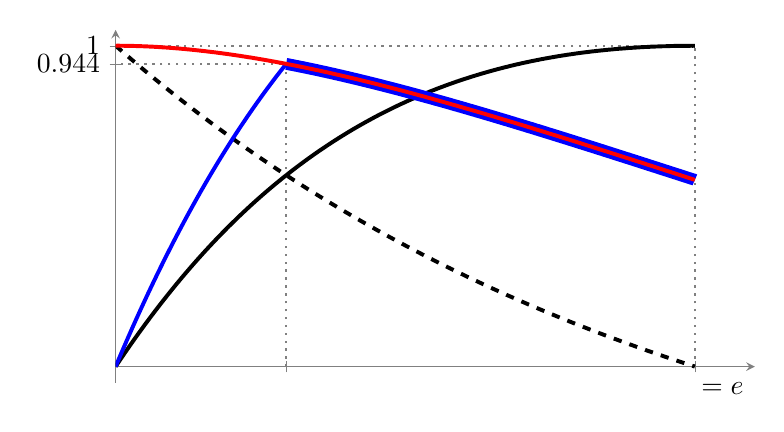
\begin{tikzpicture}[scale=1, transform shape]
\begin{axis}[
axis line style=gray,
axis lines=middle,
xlabel = {$\val$},
xtick={0, 0.800662, 2.7182818284},
ytick={0, 0.943472496484, 1},
xticklabels={0, $\fprice$, ~~~~~~$\optreserve = e$},
yticklabels={0, 0.944, $1$},
xmin=0,xmax=3.0,ymin=-0.05,ymax=1.05,
width=0.8\textwidth,
height=0.5\textwidth,
samples=500]


\addplot[dotted, gray, line width=0.3mm] (2.7182818284, 0) -- (2.7182818284, 1) -- (0, 1);
\addplot[dotted, gray, line width=0.3mm] (0.800662, 0) -- (0.800662, 0.943472496484) -- (0, 0.943472496484);

\addplot[domain=0:2.7182818284, black!100!white, line width=0.5mm] (x, {x*(exp(-x/exp(1)))});

\addplot[domain=0:2.7182818284, dashed, black!100!white, line width=0.5mm] (x, {(1+(exp(-x/exp(1))*(x+exp(1)) - 2)-x*(exp(-x/exp(1))))/1.71828182846});


\addplot[domain=0.800662:2.7182818284, blue, line width=1.5mm] (x, {(1+(exp(-x/exp(1))*(x+exp(1)) - 2)-0*x*(exp(-x/exp(1))))/1.71828182846});
\addplot[domain=0:0.800662, blue, line width=0.5mm] (x, {((1+1.71828182846)*x*(exp(-x/exp(1))))/1.71828182846});


\addplot[domain=0:2.7182818284, red, line width=0.5mm] (x, {(1+(exp(-x/exp(1))*(x+exp(1)) - 2)-0*x*(exp(-x/exp(1))))/1.71828182846});

\end{axis}

\end{tikzpicture}
    \caption{Graphical illustration of \Cref{example:all fair:mhr buyer}. The x-axis is value $\val$. 
    Consider {\FixPrice} $\mech$ with trading price $\price$ for every $\price\in[0,e]$. The black solid (resp.\ dashed) curve also represents   ${\sellerexanteutil(\mech)}/{\sellerbenchmark}$ (resp.\ ${\buyerexanteutil(\mech)}/{\buyerbenchmark}$) for the seller (resp.\ buyer). The red curve is the GFT approximation ratio ${\GFT{\mech}}/{\OPTSB}$. 
    A {\ksfair} {\FixPrice} is achieved at trading price $\fprice \approx 0.80$ with GFT approximation ratio of $0.944$. Finally, the blue curve is used in the proof of the negative result in \Cref{lem:GFT UB:mhr buyer}.}
    \label{fig:all fair:mhr buyer}
\end{figure}


\begin{lemma}
    \label{lem:GFT UB:mhr buyer}
    In \Cref{example:all fair:mhr buyer}, any BIC, IIR, ex ante WBB mechanism $\mech$ that is {\ksfair} has GFT that is less than $\fixedPriceGFTPercentageUBMHR$ of the {\SecondBest} $\OPTSB$. Here $\fixedPriceGFTPercentageUBMHR$ is the numerical evaluated upper bound of 
    \begin{align*}
        \max_{\price\in[0, e]}\frac{1}{e - 1}\cdot \left(\price\cdot e^{-\frac{\price}{e}} + \min\{(e-1)\cdot \price\cdot e^{-\frac{\price}{e}},e^{1 - \frac{\price}{e}} - 1\}\right)
    \end{align*}
\end{lemma}
The proof of \Cref{lem:GFT UB:mhr buyer} is similar to the one for \Cref{lem:GFT UB:regular buyer} in \Cref{subsec:improved GFT:regular buyer}. We first construct an upper bound of GFT (see \eqref{eq:fixed price mech suffices:mhr UB}) for every BIC, IIR, ex ante WBB, and {\ksfair} mechanisms. We then argue that in \Cref{example:all fair:mhr buyer}, a \emph{\ksfair} {\FixPrice} (which is DSIC, ex post IR, ex post SBB) optimizes this upper bound among all BIC, IIR, ex ante WBB, but (possibly not {\ksfair}) mechanisms.
\begin{proof}[Proof of \Cref{lem:GFT UB:mhr buyer}]
Fix any BIC, IIR, ex ante WBB mechanism $\mech =(\alloc,\price,\sellerprice)$ that is {\ksfair}. Let $\revratio(\mech)$ be the ratio between the buyer's expected payment over the monopoly revenue, and $\residuesurplusratio(\mech)$ be the ratio between the buyer's ex ante utility and her expected value. Namely,
\begin{align*}
    \revratio(\mech) \triangleq  
    \frac{\expect[\val]{\price(\val,0)}}{\sellerbenchmark}
    =
    \frac{\sellerexanteutil(\mech) + \expect[\val]{\price(\val,0) - \sellerprice(\val,0)}}{\sellerbenchmark} 
    \;\;
    \mbox{and}
    \;\;
    \residuesurplusratio(\mech) \triangleq \frac{\buyerexanteutil(\mech)}{\buyerbenchmark}
\end{align*}
Since mechanism $\mech$ is ex ante WBB and {\ksfair}, $\revratio(\mech) \geq \residuesurplusratio(\mech)$. Consequently, the GFT of mechanism $\mech$ can be expressed as follows:
\begin{align*}
    \GFT{\mech} 
    &= \sellerexanteutil(\mech) + \buyerexanteutil(\mech) + \expect[\val]{\price(\val,0) - \sellerprice(\val,0)}
    \\
    &=
    \revratio(\mech) \cdot \sellerbenchmark
    +
    \residuesurplusratio(\mech) \cdot \buyerbenchmark
    \\
    &=
    \revratio(\mech) \cdot \sellerbenchmark
    +
    \min\{\revratio(\mech), \residuesurplusratio(\mech)\} \cdot \buyerbenchmark
\end{align*}
where the last equality holds since $\revratio(\mech) \geq \residuesurplusratio(\mech)$ argued above. Thus, the optimal GFT among all BIC, IIR, ex ante WBB, {\ksfair} mechanisms can be upper bounded as
\begin{align}
\nonumber
    \max_{\substack{\mech\in\mechfam:~\text{$\mech$ is {\ksfair}}}} \GFT{\mech}
    & =
    \max_{\substack{\mech\in\mechfam:~\text{$\mech$ is {\ksfair}}}}  \revratio(\mech) \cdot \sellerbenchmark
    +
    \min\{\revratio(\mech), \residuesurplusratio(\mech)\} \cdot \buyerbenchmark
    \\
\label{eq:fixed price mech suffices:mhr UB}
    &\leq 
    \max_{\substack{\mech\in\mechfam}}  \revratio(\mech) \cdot \sellerbenchmark
    +
    \min\{\revratio(\mech), \residuesurplusratio(\mech)\} \cdot \buyerbenchmark
\end{align}
where we drop the {\ksfairness} requirement in the last step. 

Next we show that in \Cref{example:all fair:mhr buyer}, the optimal mechanism of the optimization program~\eqref{eq:fixed price mech suffices:mhr UB} is a {\FixPrice}. Fix an arbitrary BIC, IIR, ex ante WBB mechanism $\mech\primed = (\alloc\primed,\price\primed,\sellerprice\primed)$. Let $\val\primed$ be the unique solution such that
\begin{align*}
    \displaystyle\int_0^{\val\primed} \alloc\primed(\val) \cdot \d\buyercdf(\val) 
    =
    \displaystyle\int_{\val\primed}^{e} \left(1 - \alloc\primed(\val)\right)\cdot \d\buyercdf(\val)
\end{align*}
The existence and uniqueness of value $\val\primed$ hold, since mechanism $\mech\primed$ is BIC and thus interim allocation $\alloc\primed(\val)$ of the buyer is weakly increasing, and buyer's valuation distribution $\buyerdist$ has no point mass on $[0, e)$. Now consider the {\FixPrice} $\mech\doubleprimed$ with trading price $\price\doubleprimed \triangleq \val\primed$. We claim that $\revratio(\mech\doubleprimed) \geq \revratio(\mech\primed)$ and $\residuesurplusratio(\mech\doubleprimed) = \residuesurplusratio(\mech\primed)$.
To see this, note that 
\begin{align*}
    \revratio(\mech\doubleprimed) &\overset{(a)}{=} \frac{1}{\sellerbenchmark}\cdot \expect[\val]{\virtualval(\val)\cdot \indicator{\val\geq \price\doubleprimed}}
    =
    \frac{1}{\sellerbenchmark}\cdot 
    \left(\expect[\val]{\virtualval(\val)\cdot \indicator{\val=e}}
    +
    \displaystyle\int_{\val\primed}^{e} \virtualval(\val)\cdot \d\buyercdf(\val)
    \right)
    \\
    &\overset{(b)}{\geq}
    \frac{1}{\sellerbenchmark}\cdot 
    \left(\expect[\val]{\virtualval(\val)\cdot \indicator{\val= e}}
    +
    \displaystyle\int_{\val\primed}^{e} \virtualval(\val)\alloc\primed(\val)\cdot \d\buyercdf(\val)
    +
    \displaystyle\int_0^{\val\primed} \virtualval(\val)(1-\alloc\primed(\val))\cdot \d\buyercdf(\val)
    \right)
    \\
    &\overset{(c)}{\geq}
    \revratio(\mech\primed)
\end{align*}
where equality~(a) holds due to \Cref{prop:revenue equivalence},
inequality~(b) holds since virtual value $\virtualval(\val)$ is strictly increasing in $\val\in[0, e)$ and the construction of value $\val\primed$,
and inequality~(c) holds due to \Cref{prop:revenue equivalence} and the fact that virtual value $\virtualval(e) = e > 0$. Similarly,
\begin{align*}
    \residuesurplusratio(\mech\doubleprimed) &\overset{(a)}{=} \frac{1}{\buyerbenchmark}\cdot \expect[\val]{\buyerhazardrate(\val)\cdot \indicator{\val\geq \price\doubleprimed}}
    =
    \frac{1}{\buyerbenchmark}\cdot 
    \left(\expect[\val]{\buyerhazardrate(\val)\cdot \indicator{\val= e}}
    +
    \displaystyle\int_{\val\primed}^{e} \buyerhazardrate(\val)\cdot \d\buyercdf(\val)
    \right)
    \\
    &\overset{(b)}{=}
    \frac{1}{\buyerbenchmark}\cdot 
    \left(\expect[\val]{\buyerhazardrate(\val)\cdot \indicator{\val= e}}
    +
    \displaystyle\int_{\val\primed}^{e} \buyerhazardrate(\val)\alloc\primed(\val)\cdot \d\buyercdf(\val)
    +
    \displaystyle\int_0^{\val\primed} \buyerhazardrate(\val)(1-\alloc\primed(\val))\cdot \d\buyercdf(\val)
    \right)
    \\
    &\overset{(c)}{=}
    \residuesurplusratio(\mech\primed)
\end{align*}
where equality~(a) holds due to \Cref{prop:buyer surplus equivalence},
equality~(b) holds since hazard rate $\buyerhazardrate(\val)$ is identical for every $\val\in[0, e)$ and the construction of value $\val\primed$,
and equality~(c) holds due to \Cref{prop:buyer surplus equivalence} and the fact that hazard rate $\buyerhazardrate(e) = 0$.

Putting the two pieces together, we know that {\FixPrice} $\mech\doubleprimed$ has weakly higher objective value in program~\eqref{eq:fixed price mech suffices:mhr UB}. Hence, the optimal mechanism of the optimization program~\eqref{eq:fixed price mech suffices:mhr UB} is a {\FixPrice}. 


Finally, we evaluate the objective value of optimization program~\eqref{eq:fixed price mech suffices:mhr UB} among {\FixPrice} $\mech$ with every trading price $\price\in[0, e]$ for \Cref{example:all fair:mhr buyer} (see the blue curve in \Cref{fig:all fair:mhr buyer}). In particular, {\FixPrice} with every trading price $\price \in[0, e]$ satisfies
\begin{align*}
    \revratio(\mech) = \price \cdot e^{-\frac{\price}{e}}
    \;\;
    \mbox{and}
    \;\;
    \residuesurplusratio(\mech) = \frac{e^{1-\frac{\price}{e}} - 1}{e - 1} 
\end{align*}
Combining with the fact that $\sellerbenchmark = 1$, $\buyerbenchmark = e-1$, we know the optimal objective value of program~\eqref{eq:fixed price mech suffices:mhr UB} is upper bounded by $\fixedPriceGFTPercentageUBMHR$, with the maximum value obtained at $\price^*\approx 0.80066$. This completes the proof of \Cref{lem:GFT UB:mhr buyer}.
\end{proof}

